%%==================================================
%% chapter02.tex for SJTU Master Thesis
%% based on CASthesis
%% modified by wei.jianwen@gmail.com
%% Encoding: UTF-8
%%==================================================

\chapter{流体模拟的基本方法与框架}
\label{chap:fluidSimulation}

\section{Navier-Stokes方程组}
\label{sec:navier-stokes}

计算机图形学最有趣的问题之一是类流体行为的仿真,不同领域的对流体模拟求解的目标由不同的要求。在特效产业中,令人信服地模仿譬如烟雾、水和火等流体的外观和行为,是极其需要的;在计算机动画领域,模拟流体动画,我们更关心的是视觉效果,而不是求解的准确性,特别地,对烟而言,我们更关心烟动画中的小规模细节,而不是速度场的数值精度。在基于仿真上,流体力学被作为标准数学框架在使用。科学家们一致表示,Navier-Stokes方程式是流体流动的一个很好的数学模型。

\subsection{Navier-Stokes方程组的描述形式}

在流体力学中,Navier-Stokes方程组描述了不可压的粘性牛顿流体的方程,被称为世界上“最复杂的方程之一”。Navier-Stokes方程组的名字记录了导出该方程组的人的姓名,分别是Claude Louis Navier 和 George Gabriel Stokes,通常也可简称为N-S方程组。通常可以写成如下形式~\cite{bridson2007fluid}:

\begin{equation}
\label{basicEq}
 \frac{\partial \boldsymbol u}{\partial t} + {\boldsymbol u} \cdot \nabla {\boldsymbol u} + \frac{1}{\rho} \nabla p= {\boldsymbol g} + \upsilon \nabla \cdot \nabla {\boldsymbol u}
\end{equation}

\begin{equation}
\label{imcompressible}
 \nabla \cdot {\boldsymbol u} = 0
\end{equation}
 
\(\boldsymbol u\)表示流体的速度场。在欧拉方法中,该速度表示流体经过每个固定的点空间时所具有的速度矢量。在3D情况下,\(\boldsymbol u\)通常表示成\((u,v,w)\)的形式,分别表示3D空间标准坐标系下的\(\boldsymbol{x}, \boldsymbol{y}, \boldsymbol{z}\)三个方向上的速度大小。
 
\(p\) 表示压强场,在流体的内部,每个欧拉网格的内部都有一个压强分量。

\(t\)代表时间。
 
\(\upsilon\)代表流体的粘性系数,\(\upsilon\)越大,表示流体的粘性越大。
 
\(\rho\)表示流体的密度。
  
 \(\boldsymbol g\)表示施加在流体上的外力合力产生的加速度,这些外力包括重力、浮力等。大部分情况下,流体只受重力的影响,故在此用了通常表示重力加速度的\(\boldsymbol g\)表示。
 
 \(\nabla\)是向量空间的偏导数, 如\(\nabla {\boldsymbol u}\)表示速度场的偏导数。\(\nabla\) = (\(\frac{\partial}{\partial x}, \frac{\partial}{\partial y})\)表示2D空间的偏导,\(\nabla\) = (\(\frac{\partial}{\partial x}, \frac{\partial}{\partial y}, \frac{\partial}{\partial z})\) 则表示3D空间的偏导。另外,\(\nabla \cdot \nabla\)表示拉普拉斯算子。

\subsection{Navier-Stokes方程组的意义}
\label{sec:eqmeaning}
Navier-Stokes方程组对流体做了以下几个假设:第一,流是连续的。该假设强调液体内部不包含空隙,如溶解的气体的气泡,而且它不包含雾状粒子的聚合。第二,所有涉及到的场都是可微的,如压强场、速度场、密度和温度等。

Nacier-Stokes方程组的式~\ref{basicEq}根据质量,动量,和能量的守恒的基本原理导出。我们可以把流体模拟想象成一个粒子系统,每个粒子代表一个小水珠。那么,我们可以描述每个粒子的质量为\(m\),速度为\(\boldsymbol u\),体积为\(V\)。那么根据动量守恒定理,我们可以得到如下方程式:

\begin{equation}
\label{momentum}
 {\boldsymbol F} = m\frac{D{\boldsymbol u}}{D{t}}
\end{equation}

假设粒子受到的来自流体系统以外的力只有重力,表示为\(m{\boldsymbol g}\)。那么我们只需要分析流体粒子来自于粒子系统中其他粒子的力。

首先是压力。流体在运动的过程中,压力的作用会把高压区的流体推向低压区,从而使得流体粒子在整体上始终保持均匀分布得趋势。图\ref{pressuredepth}画出了流场内部流体粒子所有压力的示意图。从左边的图中,我们可以看出流体粒子所受的压力来自四面八方。我们假设粒子每个方向上所受的压力都相等,根据图\ref{pressuredepth}右边的示例图片,可知流体粒子的压力只与其深度有关。为了简化模型,我们用压强梯度的负值\(-\nabla p\)表示压强的不平衡效果,而\(({-\nabla p})V\)表示粒子所有到的压力。

然后是粘滞力。粘滞力总是阻碍两个粒子之间的相对运动,并且相对运动越大,粘滞力越大。这里,我们直接给出粘滞力的表达式为\(V\mu{\nabla \cdot \nabla {\boldsymbol u}}\)。其中,\(\mu\)为动态粘性系数,是流体自身的属性,通常是常量。故用重力、压力以及粘滞力表示方程式~\ref{momentum}中的外力\(\boldsymbol F\),可得到流体运动的加速度方程:

\begin{equation}
 m\frac{D{\boldsymbol u}}{D{t}} = m{\boldsymbol g} - V{\nabla p} + V{\mu}{\nabla \cdot \nabla {\boldsymbol u}}
\end{equation}

\begin{figure}
  \centering
   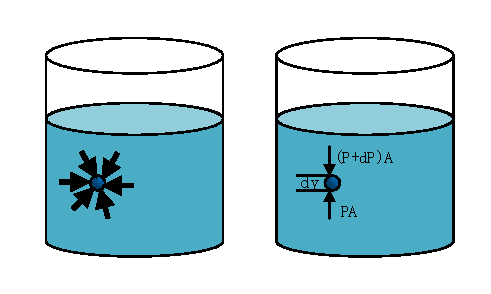
\includegraphics[height=1.8 in]{chap2/pressuredepth}
  \bicaption[pressuredepth]{}{流体粒子受压力示意图}{Fig}{Illustration of how fluid particles are affected by pressure}
\end{figure}

我们已知\(\frac{V}{m} = \frac{1}{\rho}\),设变量\(\upsilon = \frac{\mu}{\rho}\),上述方程式两边都除以粒子的质量m,则有:

展开速度场\(\boldsymbol u\)关于时间\(t\)的导数,即可得到方程式~\ref{basicEq}。

\begin{figure}
  \centering
   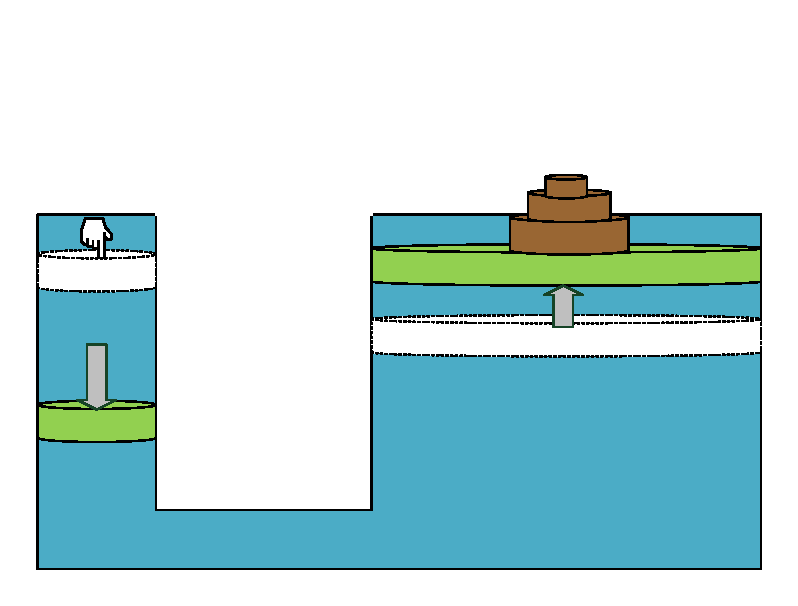
\includegraphics[height=2.3 in]{chap2/imcompressible}
  \bicaption[fig:imcompressible]{}{流体不可压示意图}{Fig}{Illustration of imcompressible condition}
\end{figure}

方程式~\ref{imcompressible}表示流体的不可压缩条件。图~\ref{fig:imcompressible}展示了流体不可压缩时的宏观表现,即压缩流体时,流体会保持其体积不变。从微观的角度讲,当我们说流体是不可压缩的时,指的是在微观时间段\(\delta t\)内,流入与流出流体任意体积为\(\Omega\)的流体表面的体积是相等的,即流体的体积变化速率为0,可以表示成如下形式:

\begin{equation}
{\iint_{\partial \Omega}}{\boldsymbol u} \cdot {\hat n} = 0 
\end{equation}

根据微积分基本定理,我们可以将上式转化为如下形式:

\begin{equation}
{\iiint_{\Omega}} \nabla \cdot {\boldsymbol u} = 0 
\end{equation}

由于上述方程式对于流体内部的任意体积\(\Omega\)都是成立的,故只有当被积函数处处为0时,上述函数积分才能为0。即为方程式~\ref{imcompressible}。

\subsection{忽略粘性力作用}

通常,在计算机动画模拟的数值计算中,会忽略掉粘性力这一项。因为相比较于其他作用力,粘性力的值通常是很小的。另外,在流体模拟的数值计算的过程中不可避免地会有数值耗散,而该数值耗散项的值的数量级与粘性力项的值的数量级比较接近,故可以近似认为数值耗散项替代了粘性力项的计算。并且从方程式~\ref{basicEq}中,我们可以看出,粘性力项的计算开销也比较大。故流体模拟的一般方法求解的是如下形式的Navier-Stokes方程组:

\begin{equation}
\label{basicEqignoreVis}
 \frac{\partial \boldsymbol u}{\partial t} + {\boldsymbol u} \cdot \nabla {\boldsymbol u} + \frac{1}{\rho} \nabla p= {\boldsymbol g}
\end{equation}

\section{流体模拟的基本方法与框架}

根据绪论部分的介绍,我们可知目前现有的流体模拟方法主要有三大类,即欧拉网格法、拉格朗日粒子法和基于旋度的方法。本文主要研究基于欧拉网格方法的重构上采样框架,故本章的该部分将会重点介绍用欧拉网格法求解Navier-Stokes方程组的框架。

\subsection{欧拉方法网格介绍}

用欧拉方法求解流体动画时,需要在网格上对其进行求解计算。Harlow等人~\cite{harlow1965numerical}提出了MAC网格方法,


